%======================================================================
\subsection{ECD plan: KiCad boards in the vault and in assemblies (23 Oct 2026, for approval)}\label{sec:ecd-plan}
%======================================================================

You asked how KiCad fits the vault: seeing boards in 3D, importing them into FreeCAD, and whether a board comes in
with proper materials. This plan answers with a test on this Mac, then proposes \eref{ECD-05} (boards in the vault)
and \eref{ECD-06} (board materials and mass) on top of \eref{ECD-01}--\eref{ECD-04}.

\paragraph{What was tested (23 Oct).} KiCad~10.0.5 is installed. Its command-line tool exported KiCad's
\emph{Arduino Mega} template board to STEP with copper, solder mask and silkscreen:
\begin{center}
\small
\texttt{kicad-cli pcb export step -{}-include-tracks -{}-include-pads -{}-include-zones}\\
\texttt{\phantom{kicad-cli pcb export step} -{}-include-silkscreen -{}-include-soldermask -o board.step board.kicad\_pcb}
\end{center}
The export took 0.8\,s (4.3\,MB). FreeCAD (this build) imported it in 0.75\,s as one \code{App::Part} with these
bodies, plus one part per connector:
\begin{center}
\small
\begin{tabular}{@{}llrl@{}}
\toprule
Body & Content & Volume & Colour\\
\midrule
\code{<board>\_PCB} & the board, 1 solid & 7\,939.6\,mm$^3$ & (0.68, 0.70, 0.57)\\
\code{<board>\_pad} & copper pads, 258 solids & 21.6\,mm$^3$ & (0.78, 0.80, 0.84)\\
\code{<board>\_soldermask} & mask, faces only & 0 & (0.28, 0.44, 0.37)\\
\code{<board>\_silkscreen} & silkscreen, faces only & 0 & white\\
\code{PinSocket\_\ldots} & connector models (KiCad library STEP) & & black, gold\\
\bottomrule
\end{tabular}
\end{center}
\textbf{So: colours come across, materials do not.} Every body's material is \emph{Default}.

\begin{figure}[!htbp]
\centering
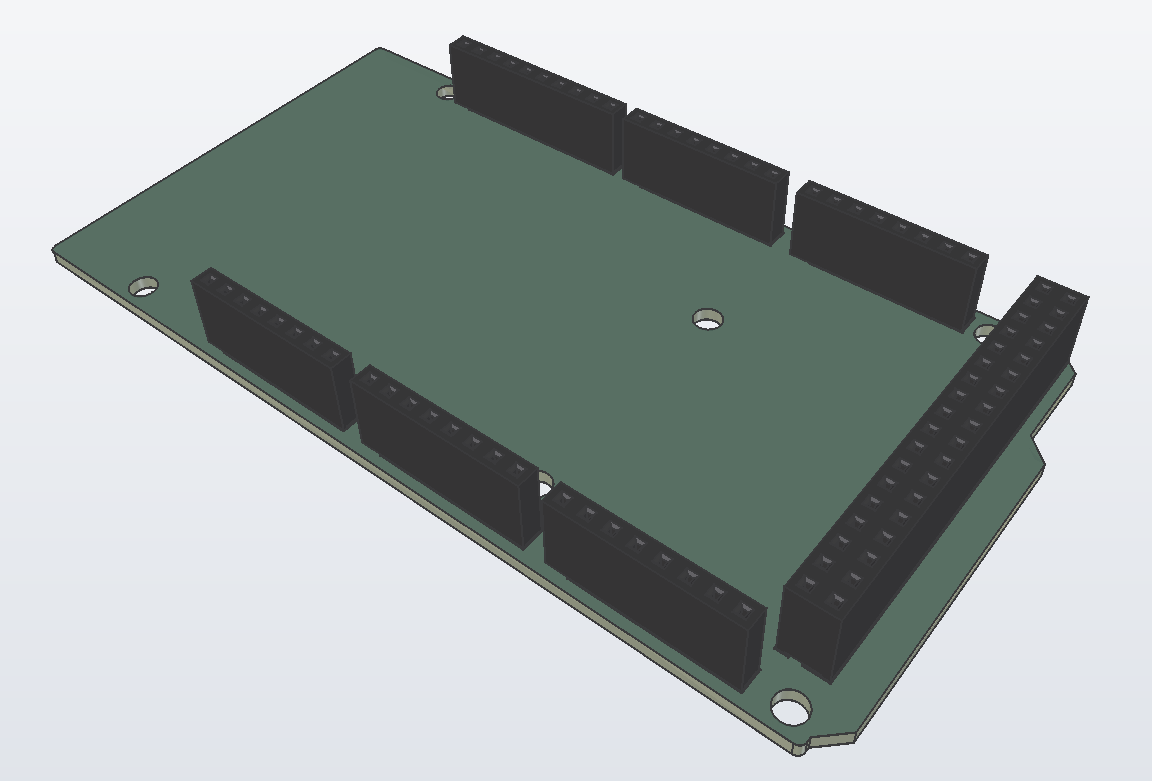
\includegraphics[width=0.49\linewidth]{fig/ecd_board_import.png}\hfill
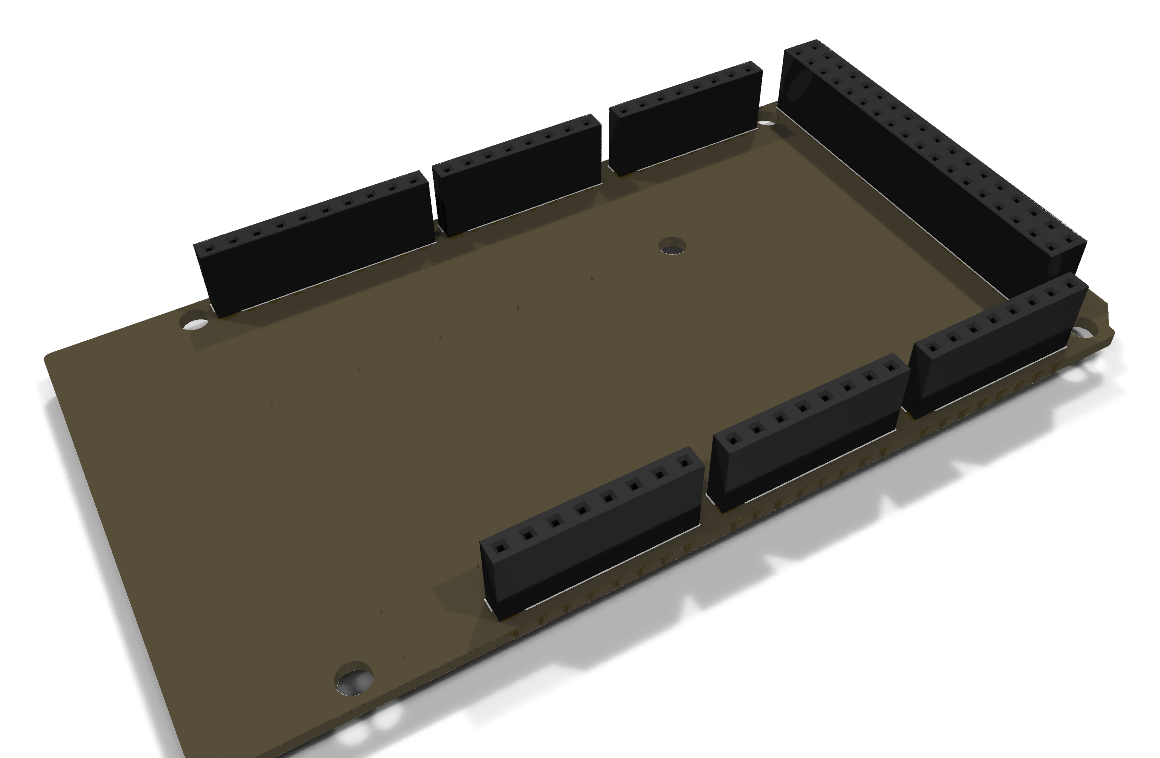
\includegraphics[width=0.49\linewidth]{fig/ecd_board_kicad.png}
\caption{\emph{Left:} the board imported into FreeCAD (this build, saved from the 3D view). \emph{Right:} the
same board rendered by KiCad itself (\code{kicad-cli pcb render}, 1.8\,s), the candidate vault thumbnail.}
\label{fig:ecd-board}
\end{figure}

Two snags, both handled by the bridge rather than by you:
\begin{itemize}[nosep]
  \item KiCad's templates name their 3D models through \code{\$\{KICAD6\_3DMODEL\_DIR\}}, which the command-line tool
        did not resolve from the environment, so the connectors were missing.
  \item \code{-{}-subst-models} swaps a STEP model in for a VRML one only when the VRML file exists; this KiCad ships
        its 3.1\,GB library as STEP only.
\end{itemize}
The bridge writes a temporary copy of the board with the model paths resolved (never your file), then exports.

%----------------------------------------------------------------------
\subsubsection*{Theory: appearance and material are two different things in FreeCAD}

A FreeCAD material carries \emph{physical} properties (density, Young's modulus, \ldots), used for mass, the
centre of gravity, the BOM and simulation, and \emph{appearance} properties used for drawing. The appearance
models are \emph{Basic Rendering} (colours, shininess, transparency), \emph{Texture Rendering} (an image mapped
onto the faces, drawn in the 3D view since FreeCAD~1.0) and \emph{Advanced Rendering} (physically based shading,
used by the Render add-on's ray tracers, not by the 3D view). The 3D view is classic Phong lighting, so it is
clear rather than photo-real. A STEP file carries colours (and names), not materials. Realistic materials
therefore come from a mapping on import, and photo-real pictures from KiCad's renderer or the Render add-on.

\paragraph{The mapping (ECD-06).} KiCad names every board body, so the rules are exact, not guesses:
\begin{center}
\small
\begin{tabularx}{\linewidth}{@{}llX@{}}
\toprule
Body & Material & Note\\
\midrule
\code{\_PCB} & FR-4 (new), $\rho = 1.85$\,g/cm$^3$ & Colour kept from KiCad (the board's stackup colour).\\
\code{\_pad}, tracks, zones & Copper, $\rho = 8.96$\,g/cm$^3$ & Finish (ENIG, HASL) as appearance, from the stackup.\\
\code{\_soldermask}, \code{\_silkscreen} & appearance only & No volume: they do not change the mass.\\
components & by footprint library & \code{Connector\_*} plastic with metal contacts, \code{Package\_*} epoxy,
  \code{Capacitor\_SMD}/\code{Resistor\_SMD} ceramic; else generic plastic (question~3).\\
\bottomrule
\end{tabularx}
\end{center}
The mass is $m = \sum_i \rho_i V_i$. For the test board: FR-4 $7\,939.6\,\text{mm}^3 \times 1.85\times10^{-3}\,
\text{g/mm}^3 = 14.7$\,g; copper pads $21.6 \times 8.96\times10^{-3} = 0.19$\,g. Library models are often hollow or
simplified, so a component's mass may also come from a small table (part number $\rightarrow$ grams) where it matters.

%----------------------------------------------------------------------
\subsubsection*{Boards in the vault (ECD-05)}

\begin{itemize}[nosep]
  \item \textbf{A PCB item type.} A KiCad project is a folder, not one file. Check-in packs the project
        (\file{.kicad\_pro}, \file{.kicad\_pcb}, \file{.kicad\_sch}, local libraries; not \file{*-backups/},
        \file{fp-info-cache} or \file{.history}) into one vault object with its own P/N, under the same ASME
        revisions as parts. Check-out unpacks it into \file{work/<user>@<mac>/<P/N>/} and \emph{Open in KiCad}
        launches KiCad on it.
  \item \textbf{Derived files at check-in.} The bridge exports the board STEP (models resolved) and renders a
        thumbnail with \code{kicad-cli pcb render} (figure~\ref{fig:ecd-board}, right). Both are stored as vault
        objects tied to that version, and made again if missing. The Data panel shows the thumbnail; the board
        never has to be opened in KiCad to be seen in 3D.
  \item \textbf{Insert board} (Design $\rightarrow$ Solid $\rightarrow$ Assemble): brings the board's STEP into the
        active assembly as one part named by its P/N, materials mapped, with a coordinate system at the board origin
        and one at each mounting hole, so joints attach to stable objects, not to faces (\eref{ECD-02}). The part
        records which board item and version it came from.
  \item \textbf{Updates.} When the vault has a newer version, the part shows the \emph{newer version} badge of
        \eref{PDM-04}. \emph{Update board} replaces the geometry inside the same part, so its placement and the
        joints on its coordinate systems survive. Theory: a joint on a coordinate system references an object
        whose name does not change, so it is immune to the toponaming problem that a joint on a face of re-imported
        geometry would hit.
\end{itemize}
The outline round trip (\eref{ECD-03}) and placement sync (\eref{ECD-04}) come after; that is where the KiCad StepUp
add-on is strongest (question~1).

%----------------------------------------------------------------------
\subsubsection*{Build order and effort}

\begin{center}
\small
\begin{tabularx}{\linewidth}{@{}lXl@{}}
\toprule
\# & Step & Effort\\
\midrule
1 & Bridge: model-path resolver, STEP export and render wrappers around \code{kicad-cli}; tests on the KiCad templates & 1\,d\\
2 & Material mapping, FR-4 and solder-mask materials, mass check (ECD-06) & 1\,d\\
3 & Insert board with its coordinate systems (ECD-02) & 1\,d\\
4 & PCB item type, project check-in and check-out, derived STEP and thumbnail (needs \eref{PDM-04}) & 2\,d\\
5 & Update board and the newer-version badge; Open in KiCad from the Data panel & 1\,d\\
\midrule
 & Total & 6\,d\\
\bottomrule
\end{tabularx}
\end{center}
Steps 1--3 do not need the vault and can start at once; steps 4--5 follow PDM-04.

%----------------------------------------------------------------------
\subsubsection*{Questions before ECD starts}

\begin{enumerate}
  \item \textbf{KiCad StepUp.} Build our own bridge on \code{kicad-cli} for import and the vault, or adopt the
        StepUp add-on (AGPL, mature outline push and pull)?\\
        \emph{Recommendation:} our own bridge for steps 1--5; evaluate StepUp only for the outline round trip.
  \item \textbf{The board in the BOM.} One line for the assembled board (PCBA) with its P/N, or the board and its
        components?\\
        \emph{Recommendation:} one PCBA line; the component BOM stays in KiCad.
  \item \textbf{Component materials.} Guess by footprint library (above), or leave components at \emph{Default} and
        count only the board?\\
        \emph{Recommendation:} guess by library, with a part-number mass table for the heavy parts.
  \item \textbf{Thumbnails.} KiCad's render (photo-like, 2\,s per board) or FreeCAD's view (matches the rest of
        the Data panel)?\\
        \emph{Recommendation:} KiCad's render.
  \item \textbf{Who edits the boards?} If someone else edits KiCad projects on another Mac, the vault's
        one-writer rule needs per-item locks to work across Macs (a later step of PDM-04).\\
        \emph{Recommendation:} confirm it is you for now.
\end{enumerate}
